% Options for packages loaded elsewhere
\PassOptionsToPackage{unicode}{hyperref}
\PassOptionsToPackage{hyphens}{url}
%
\documentclass[
  ,doc,11pt, twoside,floatsintext]{apa6}
\usepackage{amsmath,amssymb}
\usepackage{lmodern}
\usepackage{iftex}
\ifPDFTeX
  \usepackage[T1]{fontenc}
  \usepackage[utf8]{inputenc}
  \usepackage{textcomp} % provide euro and other symbols
\else % if luatex or xetex
  \usepackage{unicode-math}
  \defaultfontfeatures{Scale=MatchLowercase}
  \defaultfontfeatures[\rmfamily]{Ligatures=TeX,Scale=1}
\fi
% Use upquote if available, for straight quotes in verbatim environments
\IfFileExists{upquote.sty}{\usepackage{upquote}}{}
\IfFileExists{microtype.sty}{% use microtype if available
  \usepackage[]{microtype}
  \UseMicrotypeSet[protrusion]{basicmath} % disable protrusion for tt fonts
}{}
\makeatletter
\@ifundefined{KOMAClassName}{% if non-KOMA class
  \IfFileExists{parskip.sty}{%
    \usepackage{parskip}
  }{% else
    \setlength{\parindent}{0pt}
    \setlength{\parskip}{6pt plus 2pt minus 1pt}}
}{% if KOMA class
  \KOMAoptions{parskip=half}}
\makeatother
\usepackage{xcolor}
\IfFileExists{xurl.sty}{\usepackage{xurl}}{} % add URL line breaks if available
\IfFileExists{bookmark.sty}{\usepackage{bookmark}}{\usepackage{hyperref}}
\hypersetup{
  pdftitle={This page and the next page should be removed},
  pdflang={en-EN},
  hidelinks,
  pdfcreator={LaTeX via pandoc}}
\urlstyle{same} % disable monospaced font for URLs
\usepackage{graphicx}
\makeatletter
\def\maxwidth{\ifdim\Gin@nat@width>\linewidth\linewidth\else\Gin@nat@width\fi}
\def\maxheight{\ifdim\Gin@nat@height>\textheight\textheight\else\Gin@nat@height\fi}
\makeatother
% Scale images if necessary, so that they will not overflow the page
% margins by default, and it is still possible to overwrite the defaults
% using explicit options in \includegraphics[width, height, ...]{}
\setkeys{Gin}{width=\maxwidth,height=\maxheight,keepaspectratio}
% Set default figure placement to htbp
\makeatletter
\def\fps@figure{htbp}
\makeatother
\setlength{\emergencystretch}{3em} % prevent overfull lines
\providecommand{\tightlist}{%
  \setlength{\itemsep}{0pt}\setlength{\parskip}{0pt}}
\setcounter{secnumdepth}{-\maxdimen} % remove section numbering
% Make \paragraph and \subparagraph free-standing
\ifx\paragraph\undefined\else
  \let\oldparagraph\paragraph
  \renewcommand{\paragraph}[1]{\oldparagraph{#1}\mbox{}}
\fi
\ifx\subparagraph\undefined\else
  \let\oldsubparagraph\subparagraph
  \renewcommand{\subparagraph}[1]{\oldsubparagraph{#1}\mbox{}}
\fi
\newlength{\cslhangindent}
\setlength{\cslhangindent}{1.5em}
\newlength{\csllabelwidth}
\setlength{\csllabelwidth}{3em}
\newlength{\cslentryspacingunit} % times entry-spacing
\setlength{\cslentryspacingunit}{\parskip}
\newenvironment{CSLReferences}[2] % #1 hanging-ident, #2 entry spacing
 {% don't indent paragraphs
  \setlength{\parindent}{0pt}
  % turn on hanging indent if param 1 is 1
  \ifodd #1
  \let\oldpar\par
  \def\par{\hangindent=\cslhangindent\oldpar}
  \fi
  % set entry spacing
  \setlength{\parskip}{#2\cslentryspacingunit}
 }%
 {}
\usepackage{calc}
\newcommand{\CSLBlock}[1]{#1\hfill\break}
\newcommand{\CSLLeftMargin}[1]{\parbox[t]{\csllabelwidth}{#1}}
\newcommand{\CSLRightInline}[1]{\parbox[t]{\linewidth - \csllabelwidth}{#1}\break}
\newcommand{\CSLIndent}[1]{\hspace{\cslhangindent}#1}
\ifLuaTeX
\usepackage[bidi=basic]{babel}
\else
\usepackage[bidi=default]{babel}
\fi
\babelprovide[main,import]{english}
% get rid of language-specific shorthands (see #6817):
\let\LanguageShortHands\languageshorthands
\def\languageshorthands#1{}
% Manuscript styling
\usepackage{upgreek}
\captionsetup{font=singlespacing,justification=justified}

% Table formatting
\usepackage{longtable}
\usepackage{lscape}
% \usepackage[counterclockwise]{rotating}   % Landscape page setup for large tables
\usepackage{multirow}		% Table styling
\usepackage{tabularx}		% Control Column width
\usepackage[flushleft]{threeparttable}	% Allows for three part tables with a specified notes section
\usepackage{threeparttablex}            % Lets threeparttable work with longtable

% Create new environments so endfloat can handle them
% \newenvironment{ltable}
%   {\begin{landscape}\begin{center}\begin{threeparttable}}
%   {\end{threeparttable}\end{center}\end{landscape}}
\newenvironment{lltable}{\begin{landscape}\begin{center}\begin{ThreePartTable}}{\end{ThreePartTable}\end{center}\end{landscape}}

% Enables adjusting longtable caption width to table width
% Solution found at http://golatex.de/longtable-mit-caption-so-breit-wie-die-tabelle-t15767.html
\makeatletter
\newcommand\LastLTentrywidth{1em}
\newlength\longtablewidth
\setlength{\longtablewidth}{1in}
\newcommand{\getlongtablewidth}{\begingroup \ifcsname LT@\roman{LT@tables}\endcsname \global\longtablewidth=0pt \renewcommand{\LT@entry}[2]{\global\advance\longtablewidth by ##2\relax\gdef\LastLTentrywidth{##2}}\@nameuse{LT@\roman{LT@tables}} \fi \endgroup}

% \setlength{\parindent}{0.5in}
% \setlength{\parskip}{0pt plus 0pt minus 0pt}

% Overwrite redefinition of paragraph and subparagraph by the default LaTeX template
% See https://github.com/crsh/papaja/issues/292
\makeatletter
\renewcommand{\paragraph}{\@startsection{paragraph}{4}{\parindent}%
  {0\baselineskip \@plus 0.2ex \@minus 0.2ex}%
  {-1em}%
  {\normalfont\normalsize\bfseries\itshape\typesectitle}}

\renewcommand{\subparagraph}[1]{\@startsection{subparagraph}{5}{1em}%
  {0\baselineskip \@plus 0.2ex \@minus 0.2ex}%
  {-\z@\relax}%
  {\normalfont\normalsize\itshape\hspace{\parindent}{#1}\textit{\addperi}}{\relax}}
\makeatother

% \usepackage{etoolbox}
\makeatletter
\patchcmd{\HyOrg@maketitle}
  {\section{\normalfont\normalsize\abstractname}}
  {\section*{\normalfont\normalsize\abstractname}}
  {}{\typeout{Failed to patch abstract.}}
\patchcmd{\HyOrg@maketitle}
  {\section{\protect\normalfont{\@title}}}
  {\section*{\protect\normalfont{\@title}}}
  {}{\typeout{Failed to patch title.}}
\makeatother

\usepackage{xpatch}
\makeatletter
\xapptocmd\appendix
  {\xapptocmd\section
    {\addcontentsline{toc}{section}{\appendixname\ifoneappendix\else~\theappendix\fi\\: #1}}
    {}{\InnerPatchFailed}%
  }
{}{\PatchFailed}
\usepackage{csquotes}
\setcounter{tocdepth}{3}
\setlength{\parskip}{5pt}
\linespread{1.5}
\usepackage{setspace}
\shorttitle{}
\fancyheadoffset[L]{0pt}
\fancyhf{}
\fancyhead[RO,LE]{\small\thepage}
\renewcommand{\headrulewidth}{0pt}
\interfootnotelinepenalty=10000
\ifLuaTeX
  \usepackage{selnolig}  % disable illegal ligatures
\fi

\title{This page and the next page should be removed}
\author{\textsuperscript{}}
\date{}


\shorttitle{Subliminal Header}

\affiliation{\vspace{0.5cm}\textsuperscript{} }

\begin{document}
\maketitle

\clearpage

\mbox{}\thispagestyle{empty}\clearpage

\setcounter{page}{1}

\thispagestyle{empty}
\begin{center}
\vspace*{10mm}
\textbf{\Large An example document using RMarkdown and papaja to write your dissertation}\\

\begin{figure}[h]
\begin{center}

\includegraphics[width=!,totalheight=!,scale=0.18]{usp-brazao.jpg}
\end{center}
\end{figure}
{\setstretch{1.7} 
Inauguraldissertation\\
zur\\ 
Erlangung des Doktorgrades\\
der Humanwissenschaftlichen Fakultät\\
der Universität zu Köln  \\
nach der Prüfungsordnung vom 10.05.2010  \\
vorgelegt von  \\ 
\smallskip
\textbf{Tobias Heycke}\\
\smallskip
aus  \\
Bergisch Gladbach  \\
\smallskip
Tag der Abgabe: 01.01.1970\\
}
\end{center}

\clearpage

\mbox{}\thispagestyle{empty}\clearpage

\textbf{Acknowledgment}

\bigskip

Lorem ipsum dolor sit amet, consetetur sadipscing elitr, sed diam nonumy eirmod tempor invidunt ut labore et dolore magna aliquyam erat, sed diam voluptua. At vero eos et accusam et justo duo dolores et ea rebum. Stet clita kasd gubergren, no sea takimata sanctus est Lorem ipsum dolor sit amet. Lorem ipsum dolor sit amet, consetetur sadipscing elitr, sed diam nonumy eirmod tempor invidunt ut labore et dolore magna aliquyam erat, sed diam voluptua. At vero eos et accusam et justo duo dolores et ea rebum. Stet clita kasd gubergren, no sea takimata sanctus est Lorem ipsum dolor sit amet. Lorem ipsum dolor sit amet, consetetur sadipscing elitr, sed diam nonumy eirmod tempor danke frederik invidunt ut labore et dolore magna aliquyam erat, sed diam voluptua. At vero eos et accusam et justo duo dolores et ea rebum. Stet clita kasd gubergren, no sea takimata sanctus est Lorem ipsum dolor sit amet.

\clearpage

\mbox{}\thispagestyle{empty}\clearpage

\begin{flushleft}
{\setstretch{1.0}
\tableofcontents
}
\end{flushleft}

\newpage

\clearpage

\mbox{}\thispagestyle{empty}\clearpage

\thispagestyle{empty}

\hypertarget{summary}{%
\section{Summary}\label{summary}}

Lorem ipsum dolor sit amet, consetetur sadipscing elitr, sed diam nonumy eirmod tempor invidunt ut labore et dolore magna aliquyam erat, sed diam voluptua. At vero eos et accusam et justo duo dolores et ea rebum. Stet clita kasd gubergren, no sea takimata sanctus est Lorem ipsum dolor sit amet. Lorem ipsum dolor sit amet, consetetur sadipscing elitr, sed diam nonumy eirmod tempor invidunt ut labore et dolore magna aliquyam erat, sed diam voluptua. At vero eos et accusam et justo duo dolores et ea rebum. Stet clita kasd gubergren, no sea takimata sanctus est Lorem ipsum dolor sit amet. Lorem ipsum dolor sit amet, consetetur sadipscing elitr, sed diam nonumy eirmod tempor invidunt ut labore et dolore magna aliquyam erat, sed diam voluptua. At vero eos et accusam et justo duo dolores et ea rebum. Stet clita kasd gubergren, no sea takimata sanctus est Lorem ipsum dolor sit amet.

Duis autem vel eum iriure dolor in hendrerit in vulputate velit esse molestie consequat, vel illum dolore eu feugiat nulla facilisis at vero eros et accumsan et iusto odio dignissim qui blandit praesent luptatum zzril delenit augue duis dolore te feugait nulla facilisi. Lorem ipsum dolor sit amet, consectetuer adipiscing elit, sed diam nonummy nibh euismod tincidunt ut laoreet dolore magna aliquam erat volutpat.

Ut wisi enim ad minim veniam, quis nostrud exerci tation ullamcorper suscipit lobortis nisl ut aliquip ex ea commodo consequat. Duis autem vel eum iriure dolor in hendrerit in vulputate velit esse molestie consequat, vel illum dolore eu feugiat nulla facilisis at vero eros et accumsan et iusto odio dignissim qui blandit praesent luptatum zzril delenit augue duis dolore te feugait nulla facilisi.

Nam liber tempor cum soluta nobis eleifend option congue nihil imperdiet doming id quod mazim placerat facer possim assum. Lorem ipsum dolor sit amet, consectetuer adipiscing elit, sed diam nonummy nibh euismod tincidunt ut laoreet dolore magna aliquam erat volutpat. Ut wisi enim ad minim veniam, quis nostrud exerci tation ullamcorper suscipit lobortis nisl ut aliquip ex ea commodo consequat.\\
Duis autem vel eum iriure dolor in hendrerit in vulputate velit esse molestie consequat, vel illum dolore eu feugiat nulla facilisis.

\hypertarget{introduction}{%
\section{Introduction}\label{introduction}}

Insomnia disorder is related to dissatisfaction with duration or quality of sleep. It can be a source of distress and impairment by decreasing productivity on work or school and lowering energy to engage in social activities (Association, 2013). Prolonged effects of insomnia are associated with higher risk of harm on mental health (Johnson et al., 2006; Taylor et al., 2005) and cognitive functioning (Fortier-Brochu et al., 2012). Cognitive arousal is crucial to several behavioral models of insomnia as maintainer of the disorder (Espie et al., 2006; Harvey, 2002; Lundh, 2005; Morin et al., 1993; Ong et al., 2012; Perlis et al., 1997).

\hypertarget{dysfunctional-beliefs-and-attitudes-about-sleep}{%
\subsection{Dysfunctional beliefs and attitudes about sleep}\label{dysfunctional-beliefs-and-attitudes-about-sleep}}

Harvey's model (Harvey, 2002) is frequently mentioned as theoretical background in investigations about cognitive process in insomnia. It posits that the excess of negatively toned activity about sleep triggers arousal and distress, channeling attention and monitoring to sleep threats. This may create distorted perceptions of sleep and overestimation of the real deficits during the day. To cope, the individual may engage in safety behaviors that paradoxically increase worry and preclude sleep self correction. In Harvey's model, dysfunctional beliefs about sleep exacerbates negatively toned cognitive activity. Such beliefs are also the backbone of the Microanalytic model (Morin, 1993), one of the most cited models for insomnia in the literature (Marques et al., 2015).

Current evidence favors that beliefs and attitudes about sleep mediates insomnia perpetuation (Akram et al., 2020; Chow et al., 2018; Harvey et al., 2017; Lancee et al., 2019), although not all studies have found this association (Norell-Clarke et al., 2021). Morin (1993) suggests that insomnia maintenance feeds from a cyclic process of arousal, dysfunctional cognitions, maladaptive habits and consequences. Arousal refers to excessive activity in emotional, cognitive or physiologic domains, which can create core beliefs that guide information processing (Marques et al., 2015). This may give rise to unrealistic expectations and rigidly held beliefs about requirements for sleep, as well as increased worry about the causes and consequences of sleep disturbances. Subsequent unhealthy sleep practices may include daytime napping, excessive time in bed or indiscriminate use of sleep medication. Consequences, real or perceived, are linked to diminished performance during the day.

\hypertarget{constructs-and-their-relations}{%
\subsubsection{Constructs and Their Relations}\label{constructs-and-their-relations}}

Individuals that show stronger insomnia symptoms typically demonstrate firm endorsement of dysfunctional beliefs about sleep (Carney \& Edinger, 2006; Crönlein et al., 2014; Eidelman et al., 2016). Challenging those beliefs is in the core of Cognitive Behavioral Therapy for insomnia (CBT-I) (Belanger et al., 2006). A recent meta-analysis observed clinically significant improvements in beliefs and attitudes about sleep favoring CBT-I over controls -- although, as the authors warn, those results should be interpreted with care given the low quality of evidence (Edinger J. D. et al., 2021). Insomnia severity was identified as risk factor for anxiety (Neckelmann et al., 2007) and depression (Blanken et al., 2020; Li et al., 2016), but some studies claim this relationship the other way around (Chen et al., 2017; Jansson-Fröjmark \& Lindblom, 2008). A relationship between anxiety and depression with dysfunctional beliefs about sleep is also expected: Beck's classic cognitive mechanism for the cause and maintenance of depression gives a central role to inaccurate beliefs and maladaptive information processing (Beck, 1979). Anxiety can be elicited from displeasing memories created through exposure to adverse experiences (Brewin, 1996). Thus, unrealistic attributions and expectations about sleep (or lack of sleep) may elicit anxiety-provoking thoughts. Associação entre Depressão e DBAS (Sadler et al., 2013).

\hypertarget{measurement}{%
\subsubsection{Measurement}\label{measurement}}

To assess sleep-disruptive cognitions, Morin et al. (1993) developed the Dysfunctional Beliefs and Attitudes About Sleep Scale (DBAS). The DBAS started as a 30-item self-report instrument rated in a 100-mm visual analog scale of agreement/disagreement. Later, Morin and colleagues (2007) shortened it to a 16-item version, and replaced the response format for a 10-point scale ranging from 0 (strongly disagree) to 10 (strongly agree). The items of the brief version were selected from the original scale based on criteria of response distribution, range, item-total correlations and exploratory oblique factor analysis. A 4-factor structure was fitted to the 16 items in a confirmatory factor analysis, labeled (a) consequences of insomnia, (b) worry about sleep, (c) sleep expectations, (d) medication, and a 5th second-order general factor. The DBAS is broadly employed in experimental studies assessing sleep-related cognitions, especially the 16-item version (Thakral et al., 2020). Many researchers translated and validated the DBAS-16 across various cultures. These studies successfully replicated the original factor structure and presented good validity evidences (Boysan et al., 2010; Dhyani et al., 2013; Lang et al., 2017). Moreover, the DBAS-16 outperformed the 30 and 10-item versions in reproducibility of factor structure, measures of internal consistency, concurrent validity and sensitivity to change (Chung Ka-Fai et al., 2016).

\hypertarget{sleep-problem-acceptance-questionnaire-spaq}{%
\subsection{Sleep Problem Acceptance Questionnaire (SPAQ)}\label{sleep-problem-acceptance-questionnaire-spaq}}

\hypertarget{constructs-and-their-relations-1}{%
\subsubsection{Constructs and Their Relations}\label{constructs-and-their-relations-1}}

\hypertarget{measurement-1}{%
\subsubsection{Measurement}\label{measurement-1}}

\hypertarget{objectives}{%
\section{Objectives}\label{objectives}}

The present project therefore aims at (a) developing a Brazilian portuguese translation of the Dysfunctional Beliefs and Attitudes about Sleep Scale (DBAS-16) and Sleep Problem Acceptance Questionnaire (SPAQ), (b) examining its factorial structure, and (c) examining its construct validity.

\newpage

\hypertarget{method}{%
\section{Method}\label{method}}

\hypertarget{participants-and-study-design}{%
\subsection{Participants and Study Design}\label{participants-and-study-design}}

To estimate an adequate sample size for the confirmatory factor analyses we used MacCallum et al.'s (1996) root-mean-square error of approximation (RMSEA) tests of close and not-close fit. All tests were conducted in R version 4.1.3 (R Core Team, 2022) using \texttt{semTools} version 0.5.6 (Jorgensen et al., 2021). Morin (2007) reports RMSEA = 0.059 in a confirmatory factor analysis for DBAS-16. Taking this value as prior guess for the true RMSEA score, we calculated the sample sizes required to to reject the test for not-close fit of RMSEA \textgreater{} 0.08 and the test of close fit of RMSEA \textless{} 0.05 with a power of 0.80 and \(\alpha\) = 0.05. Results show that 216 subjects are necessary to reject the test for not-close fit, and the test of close fit would be rejected with 920 participants. Therefore, we aimed at a minimum sample size of 920 participants. SPAQ's fit index was not considered in this power analysis due to the large RMSEA (0.081) reported by the original authors (Bothelius et al., 2015).

This study was approved by the committee of ethics of the Hospital das Clínicas da Faculdade de Medicina da Universidade de São Paulo - HCFMUSP (CAAE: 46284821.1.0000.0068). To be included, participants must age between 18 and 59 years and indicate no difficulties in reading or writing. Participants will be informed about the main objective of the research and sign the informed consent. Then, they are requested to respond to an online survey using REDCap electronic data capture tools (Harris et al., 2009, 2019), including the Brazilian-Portuguese versions of DBAS-16 and SPAQ and other auxiliary instruments.

\hypertarget{item-translation}{%
\subsubsection{Item translation}\label{item-translation}}

The procedures described were applied both to Dysfunctional Beliefs and Attitudes about Sleep (DBAS-16) as well as to the SPAQ. However, the expert committee and the first translation team had a different configuration for each instrument.

In the first stage the items of the original versions were translated from English (source language) to Portuguese (target language) by three independent translators in each case, of which two were familiar with the instrument constructs and the other unaware of its concepts and with no clinical or medical background. The three versions were synthesized by an expert committee of health professionals. Then, two independent translators fluent in the source language back translated the synthesized version to English. We reconciled the back translations into a single version and submitted it to appreciation by the first author of the original questionnaire. Together with the expert committee we debated over suggestions raised by the original authors and made changes accordingly to the translated version.

As the final step, we conducted a pilot study with 15 participants from the target population to probe the pre-final version. There were 12 female participants and overall mean age was 43 years (range: 19--57 years). As to avoid restricting the feedback to specific regional contexts (Borsa et al., 2012), we aimed to diversify our sample with participants from every region of the country and with varying educational level. We were able to interview nine participants from the Southwest region, three from South, two from Northeast and one from Middle-west. We conducted individual cognitive interviews with each participant. Overall participants had a good comprehension of the test items and instructions and only a single term was replaced in DBAS-16.

\hypertarget{aditional-measures}{%
\subsection{Aditional measures}\label{aditional-measures}}

\begin{enumerate}
\def\labelenumi{\arabic{enumi}.}
\item
  \emph{Insomnia Severity Index (ISI)} (Bastien et al., 2001; Morin et al., 2011) is a 7-item questionnaire to assess insomnia severity and its impact on the patient's life. Raters use a 5-point scale raging from 0 (no problem) to 4 (very severe problem). We used the Brazilian-portuguese version (Castro, 2011).
\item
  The \emph{Hospital Anxiety and Depression Scale (HADS)} (Zigmond \& Snaith, 1983) is a scale used to assess psychological distress in non-psychiatric patients. It is formed by a two-factor structure with 7 items assessing Anxiety plus 7 items measuring Depression.
\end{enumerate}

\hypertarget{analytical-plan}{%
\subsection{Analytical Plan}\label{analytical-plan}}

\newpage

\hypertarget{partial-results}{%
\section{Partial results}\label{partial-results}}

\hypertarget{cross-cultural-adaptation}{%
\subsection{Cross-cultural adaptation}\label{cross-cultural-adaptation}}

\newpage

\hypertarget{references}{%
\section{References}\label{references}}

\setlength{\parindent}{-0.5in}
\setlength{\leftskip}{0.5in}

\hypertarget{refs}{}
\begin{CSLReferences}{1}{0}
\leavevmode\vadjust pre{\hypertarget{ref-akram2020}{}}%
Akram, U., Gardani, M., Riemann, D., Akram, A., Allen, S. F., Lazuras, L., \& Johann, A. F. (2020). Dysfunctional sleep-related cognition and anxiety mediate the relationship between multidimensional perfectionism and insomnia symptoms. \emph{Cognitive Processing}, \emph{21}(1), 141--148. \url{https://doi.org/10.1007/s10339-019-00937-8}

\leavevmode\vadjust pre{\hypertarget{ref-americanpsychiatricassociation2013}{}}%
Association, A. P. (Ed.). (2013). \emph{Diagnostic and statistical manual of mental disorders: {DSM}-5} (5th ed). {American Psychiatric Association}.

\leavevmode\vadjust pre{\hypertarget{ref-bastien2001}{}}%
Bastien, C. H., Vallières, A., \& Morin, C. M. (2001). Validation of the {Insomnia Severity Index} as an outcome measure for insomnia research. \emph{Sleep Medicine}, \emph{2}(4), 297--307. \url{https://doi.org/10.1016/s1389-9457(00)00065-4}

\leavevmode\vadjust pre{\hypertarget{ref-beck1979cognitive}{}}%
Beck, A. T. (1979). \emph{Cognitive therapy of depression}. Guilford press.

\leavevmode\vadjust pre{\hypertarget{ref-belanger2006}{}}%
Belanger, L., Savard, J., \& Morin, C. M. (2006). Clinical management of insomnia using cognitive therapy. \emph{Behavioral Sleep Medicine}, \emph{4}(3), 179--198. \url{https://doi.org/10.1207/s15402010bsm0403_4}

\leavevmode\vadjust pre{\hypertarget{ref-blanken2020}{}}%
Blanken, T. F., Borsboom, D., Penninx, B. W., \& Van Someren, E. J. (2020). Network outcome analysis identifies difficulty initiating sleep as a primary target for prevention of depression: A 6-year prospective study. \emph{Sleep}, \emph{43}(5), zsz288. \url{https://doi.org/gghm2s}

\leavevmode\vadjust pre{\hypertarget{ref-borsaAdaptacaoValidacaoInstrumentos2012}{}}%
Borsa, J. C., Damásio, B. F., \& Bandeira, D. R. (2012). {Adaptação e validação de instrumentos psicológicos entre culturas: algumas considerações}. \emph{Paidéia (Ribeirão Preto)}, \emph{22}(53), 423--432. \url{https://doi.org/10.1590/S0103-863X2012000300014}

\leavevmode\vadjust pre{\hypertarget{ref-bothelius2015}{}}%
Bothelius, K., Jernelöv, S., Fredrikson, M., McCracken, L. M., \& Kaldo, V. (2015). Measuring {Acceptance} of {Sleep Difficulties}: {The Development} of the {Sleep Problem Acceptance Questionnaire}. \emph{Sleep}, \emph{38}(11), 1815--1822. \url{https://doi.org/10.5665/sleep.5170}

\leavevmode\vadjust pre{\hypertarget{ref-boysan2010}{}}%
Boysan, M., Merey, Z., Kalafat, T., \& Kağan, M. (2010). Validation of a brief version of the dysfunctional beliefs and attitudes about sleep scale in {Turkish} sample. \emph{Procedia - Social and Behavioral Sciences}, \emph{5}, 314--317. \url{https://doi.org/10.1016/j.sbspro.2010.07.095}

\leavevmode\vadjust pre{\hypertarget{ref-brewin1996theoretical}{}}%
Brewin, C. R. (1996). Theoretical foundations of cognitive-behavior therapy for anxiety and depression. \emph{Annual Review of Psychology}, \emph{47}(1), 33--57.

\leavevmode\vadjust pre{\hypertarget{ref-carney2006}{}}%
Carney, C. E., \& Edinger, J. D. (2006). Identifying {Critical Beliefs About Sleep} in {Primary Insomnia}. \emph{Sleep}, \emph{29}(3), 342--350. \url{https://doi.org/10.1093/sleep/29.3.342}

\leavevmode\vadjust pre{\hypertarget{ref-castro}{}}%
Castro, L. S. (2011). \emph{Adaptação e validação do {Índice} de {Gravidade} de {Insônia} ({IGI})} {[}PhD thesis{]}. Universidade Federal de São Paulo.

\leavevmode\vadjust pre{\hypertarget{ref-chen2017}{}}%
Chen, P.-J., Huang, C. L.-C., Weng, S.-F., Wu, M.-P., Ho, C.-H., Wang, J.-J., Tsai, W.-C., \& Hsu, Y.-W. (2017). Relapse insomnia increases greater risk of anxiety and depression: Evidence from a population-based 4-year cohort study. \emph{Sleep Medicine}, \emph{38}, 122--129. \url{https://doi.org/10.1016/j.sleep.2017.07.016}

\leavevmode\vadjust pre{\hypertarget{ref-chow2018}{}}%
Chow, P. I., Ingersoll, K. S., Thorndike, F. P., Lord, H. R., Gonder-Frederick, L., Morin, C. M., \& Ritterband, L. M. (2018). Cognitive mechanisms of sleep outcomes in a randomized clinical trial of internet-based cognitive behavioral therapy for insomnia. \emph{Sleep Medicine}, \emph{47}, 77--85. \url{https://doi.org/10.1016/j.sleep.2017.11.1140}

\leavevmode\vadjust pre{\hypertarget{ref-chungka-fai2016}{}}%
Chung Ka-Fai, Ho Fiona Yan-Yee, \& Yeung Wing-Fai. (2016). Psychometric {Comparison} of the {Full} and {Abbreviated Versions} of the {Dysfunctional Beliefs} and {Attitudes} about {Sleep Scale}. \emph{Journal of Clinical Sleep Medicine}, \emph{12}(06), 821--828. \url{https://doi.org/10.5664/jcsm.5878}

\leavevmode\vadjust pre{\hypertarget{ref-cronlein2014}{}}%
Crönlein, T., Wagner, S., Langguth, B., Geisler, P., Eichhammer, P., \& Wetter, T. C. (2014). Are dysfunctional attitudes and beliefs about sleep unique to primary insomnia? \emph{Sleep Medicine}, \emph{15}(12), 1463--1467. \url{https://doi.org/gn3m9k}

\leavevmode\vadjust pre{\hypertarget{ref-dhyani2013}{}}%
Dhyani, M., Rajput, R., \& Gupta, R. (2013). Hindi translation and validation of dysfunctional beliefs and attitudes about sleep ({DBAS} - 16). \emph{Industrial Psychiatry Journal}, \emph{22}(1), 80--85. \url{https://doi.org/10.4103/0972-6748.123639}

\leavevmode\vadjust pre{\hypertarget{ref-edingerjackd.2021}{}}%
Edinger J. D., Arnedt J. Todd, Bertisch Suzanne M., Carney Colleen E., Harrington John J., Lichstein Kenneth L., Sateia Michael J., Troxel Wendy M., Zhou Eric S., Kazmi Uzma, Heald Jonathan L., \& Martin Jennifer L. (2021). Behavioral and psychological treatments for chronic insomnia disorder in adults: An {American Academy} of {Sleep Medicine} systematic review, meta-analysis, and {GRADE} assessment. \emph{Journal of Clinical Sleep Medicine}, \emph{17}(2), 263--298. \url{https://doi.org/10.5664/jcsm.8988}

\leavevmode\vadjust pre{\hypertarget{ref-eidelman2016}{}}%
Eidelman, P., Talbot, L., Ivers, H., BÃÂlanger, L., Morin, C. M., \& Harvey, A. G. (2016). Change in {Dysfunctional Beliefs About Sleep} in {Behavior Therapy}, {Cognitive Therapy}, and {Cognitive-Behavioral Therapy} for {Insomnia}. \emph{Behavior Therapy}, \emph{47}(1), 102--115. \url{https://doi.org/10.1016/j.beth.2015.10.002}

\leavevmode\vadjust pre{\hypertarget{ref-espie2006}{}}%
Espie, C. A., Broomfield, N. M., MacMahon, K. M. A., Macphee, L. M., \& Taylor, L. M. (2006). The attention-intention-effort pathway in the development of psychophysiologic insomnia: A theoretical review. \emph{Sleep Medicine Reviews}, \emph{10}(4), 215--245. \url{https://doi.org/10.1016/j.smrv.2006.03.002}

\leavevmode\vadjust pre{\hypertarget{ref-fortier-brochu2012}{}}%
Fortier-Brochu, E., Beaulieu-Bonneau, S., Ivers, H., \& Morin, C. M. (2012). Insomnia and daytime cognitive performance: A meta-analysis. \emph{Sleep Medicine Reviews}, \emph{16}(1), 83--94. \url{https://doi.org/10.1016/j.smrv.2011.03.008}

\leavevmode\vadjust pre{\hypertarget{ref-harris2019redcap}{}}%
Harris, P. A., Taylor, R., Minor, B. L., Elliott, V., Fernandez, M., O'Neal, L., McLeod, L., Delacqua, G., Delacqua, F., Kirby, J.others. (2019). The REDCap consortium: Building an international community of software platform partners. \emph{Journal of Biomedical Informatics}, \emph{95}, 103208.

\leavevmode\vadjust pre{\hypertarget{ref-harris2009research}{}}%
Harris, P. A., Taylor, R., Thielke, R., Payne, J., Gonzalez, N., \& Conde, J. G. (2009). Research electronic data capture (REDCap)---a metadata-driven methodology and workflow process for providing translational research informatics support. \emph{Journal of Biomedical Informatics}, \emph{42}(2), 377--381.

\leavevmode\vadjust pre{\hypertarget{ref-harvey2002}{}}%
Harvey, A. G. (2002). A cognitive model of insomnia. \emph{Behaviour Research and Therapy}, \emph{40}(8), 869--893. \url{https://doi.org/fwxq35}

\leavevmode\vadjust pre{\hypertarget{ref-harvey2017}{}}%
Harvey, A. G., Dong, L., Bélanger, L., \& Morin, C. M. (2017). Mediators and treatment matching in behavior therapy, cognitive therapy and cognitive behavior therapy for chronic insomnia. \emph{Journal of Consulting and Clinical Psychology}, \emph{85}(10), 975--987. \url{https://doi.org/10.1037/ccp0000244}

\leavevmode\vadjust pre{\hypertarget{ref-jansson-frojmark2008b}{}}%
Jansson-Fröjmark, M., \& Lindblom, K. (2008). A bidirectional relationship between anxiety and depression, and insomnia? {A} prospective study in the general population. \emph{Journal of Psychosomatic Research}, \emph{64}(4), 443--449. \url{https://doi.org/10.1016/j.jpsychores.2007.10.016}

\leavevmode\vadjust pre{\hypertarget{ref-johnson2006}{}}%
Johnson, E. O., Roth, T., \& Breslau, N. (2006). The association of insomnia with anxiety disorders and depression: Exploration of the direction of risk. \emph{Journal of Psychiatric Research}, \emph{40}(8), 700--708. \url{https://doi.org/d5k6f6}

\leavevmode\vadjust pre{\hypertarget{ref-semtools}{}}%
Jorgensen, T. D., Pornprasertmanit, S., Schoemann, A. M., \& Rosseel, Y. (2021). \emph{\texttt{semTools}: {U}seful tools for structural equation modeling}. \url{https://CRAN.R-project.org/package=semTools}

\leavevmode\vadjust pre{\hypertarget{ref-lancee2019}{}}%
Lancee, J., Effting, M., van der Zweerde, T., van Daal, L., van Straten, A., \& Kamphuis, J. H. (2019). Cognitive processes mediate the effects of insomnia treatment: Evidence from a randomized wait-list controlled trial. \emph{Sleep Medicine}, \emph{54}, 86--93. \url{https://doi.org/10.1016/j.sleep.2018.09.029}

\leavevmode\vadjust pre{\hypertarget{ref-lang2017}{}}%
Lang, C., Brand, S., Holsboer-Trachsler, E., Pühse, U., Colledge, F., \& Gerber, M. (2017). Validation of the {German} version of the short form of the dysfunctional beliefs and attitudes about sleep scale ({DBAS-16}). \emph{Neurological Sciences}, \emph{38}(6), 1047--1058. \url{https://doi.org/10.1007/s10072-017-2921-x}

\leavevmode\vadjust pre{\hypertarget{ref-li2016}{}}%
Li, L., Wu, C., Gan, Y., Qu, X., \& Lu, Z. (2016). Insomnia and the risk of depression: A meta-analysis of prospective cohort studies. \emph{BMC Psychiatry}, \emph{16}, 375. \url{https://doi.org/f9bsxr}

\leavevmode\vadjust pre{\hypertarget{ref-lundh2005}{}}%
Lundh, L.-G. (2005). The {Role} of {Acceptance} and {Mindfulness} in the {Treatment} of {Insomnia}. \emph{Journal of Cognitive Psychotherapy}, \emph{19}(1), 29--39. \url{https://doi.org/10.1891/jcop.19.1.29.66331}

\leavevmode\vadjust pre{\hypertarget{ref-maccallum1996}{}}%
MacCallum, R. C., Browne, M. W., \& Sugawara, H. M. (1996). Power analysis and determination of sample size for covariance structure modeling. \emph{Psychological Methods}, \emph{1}(2), 130--149. \url{https://doi.org/10.1037/1082-989X.1.2.130}

\leavevmode\vadjust pre{\hypertarget{ref-marques2015}{}}%
Marques, D. R., Allen Gomes, A., Clemente, V., Santos, J. M., \& Castelo-Branco, M. (2015). Hyperarousal and failure to inhibit wakefulness in primary insomnia: "``Birds of a feather"? \emph{Sleep and Biological Rhythms}, \emph{13}(3), 219--228. \url{https://doi.org/10.1111/sbr.12115}

\leavevmode\vadjust pre{\hypertarget{ref-morin1993insomnia}{}}%
Morin, C. M. (1993). \emph{Insomnia: Psychological assessment and management.} Guilford press.

\leavevmode\vadjust pre{\hypertarget{ref-morin2011a}{}}%
Morin, C. M., Belleville, G., Bélanger, L., \& Ivers, H. (2011). \href{https://www.ncbi.nlm.nih.gov/pmc/articles/PMC3079939}{The {Insomnia Severity Index}: {Psychometric Indicators} to {Detect Insomnia Cases} and {Evaluate Treatment Response}}. \emph{Sleep}, \emph{34}(5), 601--608.

\leavevmode\vadjust pre{\hypertarget{ref-morin1993}{}}%
Morin, C. M., Stone, J., Trinkle, D., Mercer, J., \& Remsberg, S. (1993). Dysfunctional beliefs and attitudes about sleep among older adults with and without insomnia complaints. \emph{Psychology and Aging}, \emph{8}(3), 463--467. \url{https://doi.org/frwwvp}

\leavevmode\vadjust pre{\hypertarget{ref-morin2007a}{}}%
Morin, C. M., Vallières, A., \& Ivers, H. (2007). Dysfunctional {Beliefs} and {Attitudes} about {Sleep} ({DBAS}): {Validation} of a {Brief Version} ({DBAS-16}). \emph{Sleep}, \emph{30}(11), 1547--1554. \url{https://doi.org/10.1093/sleep/30.11.1547}

\leavevmode\vadjust pre{\hypertarget{ref-neckelmann2007}{}}%
Neckelmann, D., Mykletun, A., \& Dahl, A. A. (2007). Chronic insomnia as a risk factor for developing anxiety and depression. \emph{Sleep}, \emph{30}(7), 873--880. \url{https://doi.org/gf26g2}

\leavevmode\vadjust pre{\hypertarget{ref-norell-clarke2021}{}}%
Norell-Clarke, A., Hagström, M., \& Jansson-Fröjmark, M. (2021). Sleep-{Related Cognitive Processes} and the {Incidence} of {Insomnia Over Time}: {Does Anxiety} and {Depression Impact} the {Relationship}? \emph{Frontiers in Psychology}, \emph{12}. \url{https://doi.org/gk8x3v}

\leavevmode\vadjust pre{\hypertarget{ref-ong2012}{}}%
Ong, J. C., Ulmer, C. S., \& Manber, R. (2012). Improving sleep with mindfulness and acceptance: {A} metacognitive model of insomnia. \emph{Behaviour Research and Therapy}, \emph{50}(11), 651--660. \url{https://doi.org/f4fczt}

\leavevmode\vadjust pre{\hypertarget{ref-perlis1997}{}}%
Perlis, M. L., Giles, D. E., Mendelson, W. B., Bootzin, R. R., \& Wyatt, J. K. (1997). Psychophysiological insomnia: The behavioural model and a neurocognitive perspective. \emph{Journal of Sleep Research}, \emph{6}(3), 179--188. \url{https://doi.org/fcrnvj}

\leavevmode\vadjust pre{\hypertarget{ref-R-base}{}}%
R Core Team. (2022). \emph{R: A language and environment for statistical computing}. R Foundation for Statistical Computing. \url{https://www.R-project.org/}

\leavevmode\vadjust pre{\hypertarget{ref-sadler2013}{}}%
Sadler, P., McLaren, S., \& Jenkins, M. (2013). A psychological pathway from insomnia to depression among older adults. \emph{International Psychogeriatrics}, \emph{25}(8), 1375--1383. \url{https://doi.org/10.1017/S1041610213000616}

\leavevmode\vadjust pre{\hypertarget{ref-taylor2005}{}}%
Taylor, D. J., Lichstein, K. L., Durrence, H. H., Reidel, B. W., \& Bush, A. J. (2005). Epidemiology of {Insomnia}, {Depression}, and {Anxiety}. \emph{Sleep}, \emph{28}(11), 1457--1464. \url{https://doi.org/gg5k3t}

\leavevmode\vadjust pre{\hypertarget{ref-thakral2020}{}}%
Thakral, M., Von Korff, M., McCurry, S. M., Morin, C. M., \& Vitiello, M. V. (2020). Changes in dysfunctional beliefs about sleep after cognitive behavioral therapy for insomnia: {A} systematic literature review and meta-analysis. \emph{Sleep Medicine Reviews}, \emph{49}, 101230. \url{https://doi.org/10.1016/j.smrv.2019.101230}

\leavevmode\vadjust pre{\hypertarget{ref-zigmond1983hospital}{}}%
Zigmond, A. S., \& Snaith, R. P. (1983). The hospital anxiety and depression scale. \emph{Acta Psychiatrica Scandinavica}, \emph{67}(6), 361--370.

\end{CSLReferences}


\clearpage

\begin{appendix}
\section{Sets of IADS sounds used in Experiment 1: Valence Positive,
Neutral,
Negative}\label{sets-of-iads-sounds-used-in-experiment-1-valence-positive-neutral-negative}

\begin{table}[h]
\begin{center}
\begin{threeparttable}
\caption{\label{tab:appendix_table}Sound-Nr. (Bradley \& Lang, 2007)}
\begin{tabular}{ccc}
\toprule
Positive & \multicolumn{1}{c}{Neutral} & \multicolumn{1}{c}{Negative}\\
\midrule
110 & 109 & 278\\
172 & 171 & 279\\
725 & 206 & 285\\
809 & 221 & 296\\
810 & 270 & 501\\
811 & 365 & 624\\
815 & 367 & 625\\
816 & 368 & 711\\
817 & 375 & 712\\
820 & 722 & 719\\
\bottomrule
\end{tabular}
\end{threeparttable}
\end{center}
\end{table}

\clearpage

\section{Priors for the Bayesian logistic mixed effects regression
models of two-alternative forced choice
responses}\label{priors-for-the-bayesian-logistic-mixed-effects-regression-models-of-two-alternative-forced-choice-responses}

\begin{figure}[!h]
\centering
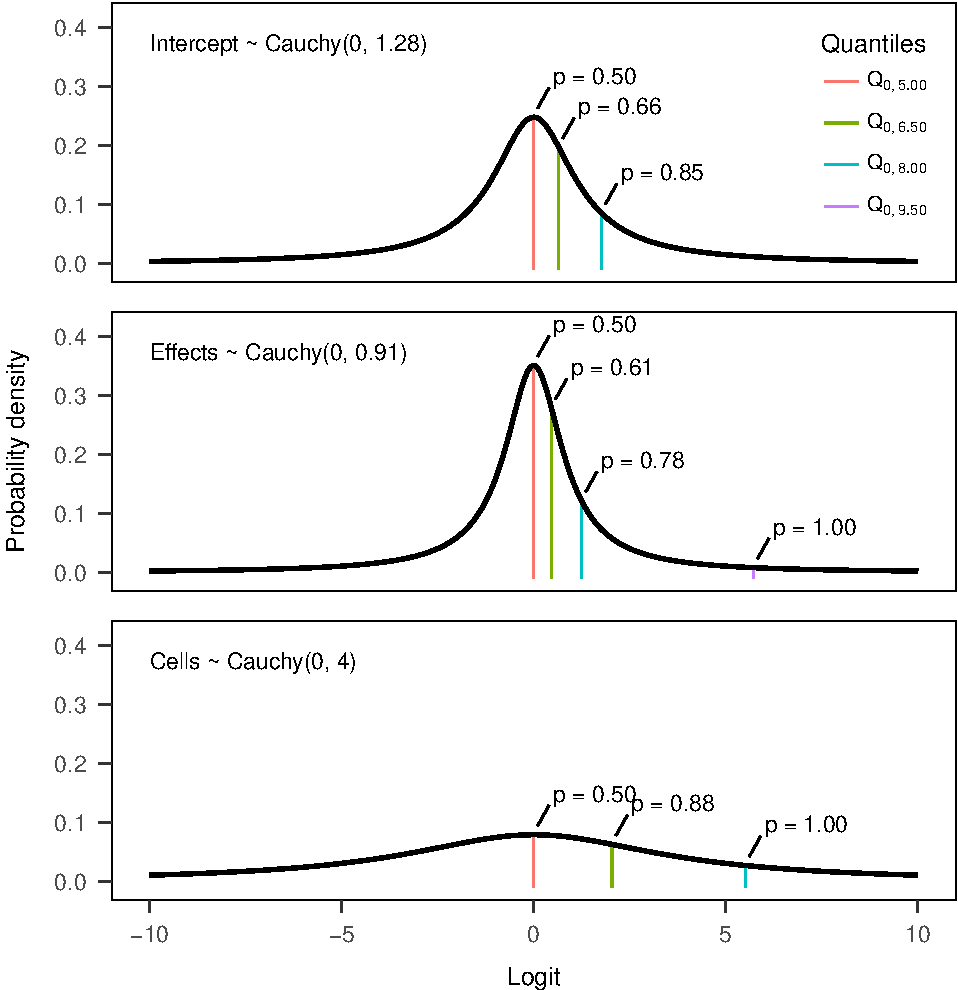
\includegraphics{Chapter02_files/figure-latex/appendix-figure-1.pdf}
\caption{\label{fig:appendix-figure}Priors for the Bayesian logistic mixed
effects regression models of two-alternative forced choice responses.
Colored lines represent distribution quantiles; annoted probabilities
represent the resulting probability of choosing a positively paired CS
starting from chance level (p = 0.5).}
\end{figure}

\clearpage

\section{Mean CS visibility (Experiment 2 and Experiment
3)}\label{mean-cs-visibility-experiment-2-and-experiment-3}

Mean Visibility scores of each CS in Experiment 2 (chance level = .250,
\(N = 37\)) and pilot of Experiment 3 (chance level = .125, \(N = 7\))
and the presentation time for each stimulus as used in Experiment 3.

\begin{table}[h]
\begin{center}
\begin{threeparttable}
\caption{\label{tab:appendix_table2}Mean CS visibility}
\begin{tabular}{cccc}
\toprule
CS & \multicolumn{1}{c}{Visibility Study 2} & \multicolumn{1}{c}{Visibility Pilot} & \multicolumn{1}{c}{Set}\\
\midrule
03.png & .512 & .400 & 1000 ms\\
08.png & .540 & .329 & 1000 ms\\
14.png & .900 & .657 & 1000 ms\\
22.png & .475 & .400 & 1000 ms\\
04.png & .438 & .200 & 20 ms\\
20.png & .400 & .271 & 20 ms\\
50.png & .356 & .129 & 20 ms\\
51.png & .423 & .243 & 20 ms\\
\bottomrule
\end{tabular}
\end{threeparttable}
\end{center}
\end{table}
\end{appendix}

\end{document}
